\documentclass{article}
\usepackage{mathtools}
\usepackage{amssymb}
\usepackage{float}
\begin{document}
\centerline{\sc \large Particle \& Collision Simulation}
\centerline{Course Notes from Fundamentals of Computer Animation Comp559 with Paul Kry.}

\section{Mathematical background}
\subsection{The gradient, the Hessian and the Jacobian}
The gradient $\nabla f$ of  a function $ f: \mathbb{R}^n \longrightarrow \mathbb{R} $
is the row (sometimes column?) vector of its partial derivatives:
\[
    \nabla f =
    \begin{pmatrix}
        \dfrac{\partial f}{\partial x_1} &
        \dfrac{\partial f}{\partial x_2} &
        \hdots &
        \dfrac{\partial f}{\partial x_n}
    \end{pmatrix}
\]
Applied over the whole domain of $f$, It represents a vector field that points in the direction of the greatest rate of increase of the scalar field,
and whose magnitude is the greatest rate of change.


Similarly, the Hessian $\nabla ^2 f$ of a function $ f: \mathbb{R}^n \longrightarrow \mathbb{R} $
is the square matrix of its second partial derivatives:
\[
    \nabla ^2 f =
    \begin{bmatrix}
        \frac{\partial^2 f}{\partial x_1^2} & \frac{\partial^2 f}{\partial x_1\,\partial x_2} & \cdots & \frac{\partial^2 f}{\partial x_1\,\partial x_n} \\ \\
        \frac{\partial^2 f}{\partial x_2\,\partial x_1} & \frac{\partial^2 f}{\partial x_2^2} &  & \frac{\partial^2 f}{\partial x_2\,\partial x_n} \\ \\
        \vdots &   & \ddots & \vdots \\ \\
        \frac{\partial^2 f}{\partial x_n\,\partial x_1} & \frac{\partial^2 f}{\partial x_n\,\partial x_2} & \cdots & \frac{\partial^2 f}{\partial x_n^2}
    \end{bmatrix}
\]
We can derive the Hessian by taking $\nabla(\nabla f)$ where the gradient of $f$ is expressed as a row vector:
\[
    \nabla(\nabla f) = \nabla (
    \begin{bmatrix}
        \dfrac{\partial f_1}{\partial x_1} & \dfrac{\partial f_1}{\partial x_2}
    \end{bmatrix}) =
    \begin{bmatrix}
        \dfrac{\partial }{\partial x_1} \\ \\
        \dfrac{\partial }{\partial x_2}
    \end{bmatrix} \cdot
    \begin{bmatrix}
        \dfrac{\partial f_1}{\partial x_1} & \dfrac{\partial f_1}{\partial x_2}
    \end{bmatrix} =
    \begin{bmatrix}
        \dfrac{\partial^2 f_1}{\partial^2 x_1} & \dfrac{\partial^2 f_1}{\partial x_1 \partial x_2} \\ \\
        \dfrac{\partial^2 f_1}{\partial x_2 \partial x_1} & \dfrac{\partial^2 f_1}{\partial^2 x_2^2}
    \end{bmatrix}
\]


The Jacobian $J f$ of a function $ f: \mathbb{R}^n \longrightarrow \mathbb{R}^m $
is a matrix of its partial derivatives:
\[
    Jf=
    \begin{bmatrix}
        \dfrac{\partial f_1}{\partial x_1} & \dfrac{\partial f_1}{\partial x_2} & \cdots & \dfrac{\partial f_1}{\partial x_n} \\ \\
        \dfrac{\partial f_2}{\partial x_1} & \dfrac{\partial f_2}{\partial x_2} &   & \dfrac{\partial f_2}{\partial x_n} \\ \\
        \vdots &  & \ddots & \vdots \\ \\
        \dfrac{\partial f_m}{\partial x_1} & \dfrac{\partial f_m}{\partial x_2} & \cdots & \dfrac{\partial f_m}{\partial x_n}
    \end{bmatrix}
\]
Note that each row of $J$ is the gradient of $f$: $J_{(i, :)} = \nabla f_i(x)$.

\subsubsection{Relationship between the Hessian and the Jacobian}
Example: ``The Jacobian of the force is the Hessian of the energy.''
First, let us define an \underline{energy} function $V : \mathbb{R}^2 \rightarrow \mathbb{R}$ which yields a potential energy value for each point in the space (a scalar field). We also define a \underline{force} function $F : \mathbb{R}^2 \rightarrow \mathbb{R}^2$ which yields a force vector field.

We can obtain the force field by computing the gradient of the energy field.
\[
    F = \nabla V =
    \begin{pmatrix}
        \dfrac{\partial V}{\partial x_1} &
        \dfrac{\partial V}{\partial x_2}
    \end{pmatrix} = 
    \begin{pmatrix} f_1 & f_2 \end{pmatrix}
\]
Now the Hessian of the energy:
\[
    \nabla^2 V =
    \begin{bmatrix}
        \dfrac{\partial^2 V}{\partial^2 x_1} & \dfrac{\partial^2 V}{\partial x_1 \partial x_2}  \\ \\
        \dfrac{\partial^2 V}{\partial x_1 \partial x_2} & \dfrac{\partial^2 V}{\partial^2 x_2}
    \end{bmatrix}
\]
The Jacobian of the force:
\[
    J F =
    \begin{bmatrix}
        \dfrac{\partial f_1}{\partial x_1} & \dfrac{\partial f_1}{\partial x_2} \\ \\
        \dfrac{\partial f_2}{\partial x_1} & \dfrac{\partial f_2}{\partial x_2}
    \end{bmatrix} = 
    \begin{bmatrix}
        \dfrac{\partial}{\partial x_1} \cdot \dfrac{\partial V}{\partial x_1} &
        \dfrac{\partial}{\partial x_2} \cdot \dfrac{\partial V}{\partial x_1} \\ \\
        \dfrac{\partial}{\partial x_1} \cdot \dfrac{\partial V}{\partial x_2} &
        \dfrac{\partial}{\partial x_2} \cdot \dfrac{\partial V}{\partial x_2}
    \end{bmatrix} = 
    \begin{bmatrix}
        \dfrac{\partial^2 V}{\partial^2 x_1} & \dfrac{\partial^2 V}{\partial x_1 \partial x_2}  \\ \\
        \dfrac{\partial^2 V}{\partial x_1 \partial x_2} & \dfrac{\partial^2 V}{\partial^2 x_2}
    \end{bmatrix} = \nabla^2 V
\]
Thus, if the vector-valued function taken by the Jacobian is the gradient of a scalar-valued function $S(\mathbf{x})$, then this specific Jacobian is equivalent to the Hessian of $S(\mathbf{x})$.
\subsection{Taylor expansion}
The taylor serie of an infinitely differentiable function $f$ at $x=a$ is given by:
\[
f(x) = \sum_{k=0}^{+\infty} \frac{f^{(k)}(a)}{k!}(x-a)^k
\]
A finite number of terms can be used as an approximation function of $f$ around $a$.
For a k-differentiable function, Taylor's theorem states that:
\begin{align*}
    f(x) &= f(a) + f'(a)(x-a) + \frac{f''(a)}{2!}(x-a)^2 + \cdots \\ &\qquad {} +\frac{f^{(k)}(a)}{k!}(x-a)^k + h_k(x)(x-a)^k \\
    f(x) &= P_k(x) + h_k(x)(x-a)^k \\
    f(x) &= P_k(x) + R_k(x)
\end{align*} where $lim_{x\to a}h_k(x)=0$. \newline
The remainder term $R_k(x) = h_k(x)(x-a)^k = o(|x-a|^k),  x \longrightarrow a$ represents the approximation error.

Thus, say we have a function $x(t+h)$. We then can approximate it around $t$ using its Taylor expansion:
\begin{align*}
    x(t+h) &= x(t) + x'(t)((t+h)-t) + \frac{x''(h)}{2!}((t+h)-t)^2 + \cdots \\ &\qquad {} +\frac{x^{(k)}(h)}{k!}((t+h)-t)^k + h_k(t)((t+h)-t)^k \\
    x(t+h) &= x(t) + h x'(t) + \frac{h^2}{2!}x''(h)+ \cdots + \frac{h^k}{k!}x^{(k)}(h) +  h^k h_k(t) 
\end{align*}
We will later use this expansion as a position update formula ($x$ will be the position and $h<1$ the timestep).

\subsection{Taylor expansion for multivariate or vector functions} 
Very often in our computations, we will use vector/matrix-form values --- position, velocity and acceleration are all vectors.
Hence, we can try to derive an Taylor expansion approximation of second-order for a vector function.
\begin{align}
    y=f(\mathbf{x}+\Delta\mathbf{x})\approx f(\mathbf{x}) + J(\mathbf{x})\Delta \mathbf{x} +\frac{1}{2} \Delta\mathbf{x}^\mathrm{T} H(\mathbf{x}) \Delta\mathbf{x}
\end{align}
\section{Particle simulation}
In physically based animation, particles can be divided into two main groups:
\begin{itemize}
\item Non-interacting particles such as dust, sparks, snow, rain, \ldots 
\item Interacting particles such as cloth, cables, elastic solids, dluids, \ldots 
\end{itemize}
\subsection{Introductory example}
Say we have snow blown by a simple wind force function $f(x, t)$ which depends on both time and position:
\[\dot{x} = f(x, t)\]
In solving an ODE such as this one, we might have a boundary value problem where knowing the starting point $x_0$ and the ending point $x_n$, we look for $x(t)$. This is usually hard to compute and can have many possible solutions (i.e. cycles). We could also have an initial value problem: we know $x_0$ (and $\dot{x_0}$), and we want to compute $x(t)$. This method is generally faster.
\begin{align*}
    \mathbf{x} = \begin{bmatrix} x \\ y \end{bmatrix}&, \quad
    \mathbf{\dot{x}} = \begin{bmatrix} \dot{x} \\ \dot{y} \end{bmatrix} = \begin{bmatrix} 1 \\ -3y \end{bmatrix}, \quad
    \mathbf{x} \in \mathbb{R} \\
    \dot{x} = 1,\quad \dot{y} = -3y \quad &\Rightarrow \quad x(t) = c_1+t, \quad y(t) = c_2 e^{-3 x} \\
    \mathbf{x_0} = \begin{bmatrix} 0 \\ 1 \end{bmatrix} \quad &\Rightarrow \quad 
    x(t) = t, \quad y(t) = e^{-3 x}
\end{align*}
However, computing the exact formula for a particle path would generally be unrealistic. The only viable approach is to approximate the ODE solution by discretizing time. The particle path $x(t)$ will then describe a discrete sequence of displacements --- hopefully small enough so that they remain unnoticeable. Correct appearance and expected behavior are our primary concerns.
\subsection{Forward Euler}
Using the forward euler approximation method, we discretize time and find solution at each time steps $0<h<1$. For all the methods we will explore, the size of $h$ will be an important component to the stability of the approximation. Very often, time steps too large will cause the particle system to 'blow up'.
\[\mathbf{x}_0, \mathbf{x}_1, \mathbf{x}_2, \ldots = \mathbf{x}(0),\mathbf{x}(h), \mathbf{x}(2h), \ldots \mbox{ for small h, so that } \mathbf{x}(t+h) = \mathbf{x}_{k+1}\]
\begin{align}
    \mathbf{x}_{k+1} &= \mathbf{x}_k + h \mathbf{\dot{x}}_k \\
                     &= \mathbf{x}_k + h f(\mathbf{x}_k, t) 
\end{align}
We can also see it as a first derivative approximation:
\begin{align}
    \mathbf{\dot{x}}_k &\approx \frac{\mathbf{x}_{k+1}-\mathbf{x}_k}{h}
\end{align}
Or using the taylor expansion:
\begin{align}
    \mathbf{x}(t+h) &= \mathbf{x}(t) + h \mathbf{x}'(t) + \frac{h^2}{2!}\mathbf{x}''(h)+ \cdots + \frac{h^k}{k!}\mathbf{x}^{(k)}(h) +  h^k h_k(t) \\
    &= \mathbf{x}(t) + h \mathbf{\dot{x}}(t) + O(h^2)
\end{align}
\section{Collision Detection}
\subsection{Lagrange Multiplier}
Recall that a Lagrange Multiplier $\lambda$ is defined as follows:
\begin{equation}
\nabla f(x_0, y_0, z_0) = \lambda \cdot \nabla g(x_0, y_0, z_0)
\end{equation}
where $(x_0, y_0, z_0)$ is the maxima or the minima of a function $f$ subject to a constraint $g$. It is easier to gain intuition when the domain of $f$ is $\mathbb{R}^2$. Both $f : \mathbb{R}^2 \rightarrow \mathbb{R}$ and $g : \mathbb{R}^2 \rightarrow \mathbb{R}$ are standard scalar-valued functions mapping a plane position to a height value, generating a surface in 3d space. However, setting $g(x,y)=c$ effectively restricts the domain to a 2d contour line. Moving along the contour line $g=c$, the value of f can vary. However, an extremum of $f$ will be reached when no variation occurs (at a stationary point). This happens only when the contour line for $g=c$ meets contour lines of $f$ tangentially, or equivalently when the gradients at this point are parallel. This is equivalent to the Lagrange Multiplier equation where $\lambda$ simply is a scaling factor between two parallel gradient vectors.
\begin{figure}[H]
    \centering
    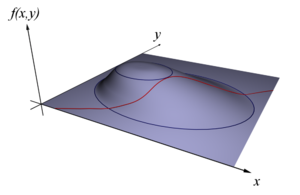
\includegraphics[scale=0.7]{LagrangeMultipliers3D.png}
    \caption{Find x and y to maximize f(x,y) subject to a constraint (shown in red) g(x,y) = c.}
\end{figure}
\begin{figure}[H]
    \centering
    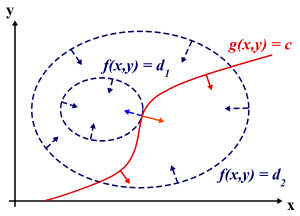
\includegraphics[scale=0.6]{LagrangeMultipliers2D.png}
    \caption{Contour map. The red line shows the constraint g(x,y) = c. The blue lines are contours of f(x,y). The point where the red line tangentially touches a blue contour is our solution.}
\end{figure}
As an example, say we want to maximize the volume of a box without a cover, using 12 unit squared of material. We must then maximize $f(x,y,z) = xyz $ (the volume) under the constraint $g(x,y,z) = 2xz + 2yz + xy - 12 = 0$ (the surface). Under the Lagrange multiplier method, we look for values of x, y and z such that $\nabla f = \lambda \nabla g$ and $g(x,y,z) = 0$. Thus, we have the following system of equations:
\begin{equation}
\begin{pmatrix}
    \dfrac{\partial f}{\partial x} \\ \\ \dfrac{\partial f}{\partial y} \\ \\ \dfrac{\partial f}{\partial z}
\end{pmatrix} = 
\lambda \cdot
\begin{pmatrix}
    \dfrac{\partial g}{\partial x} \\ \\ \dfrac{\partial g}{\partial y} \\ \\ \dfrac{\partial g}{\partial z}
\end{pmatrix} \implies 
\begin{pmatrix}
    yz \\ xz \\ xy
\end{pmatrix} = 
\lambda \cdot
\begin{pmatrix}
    2z+y \\ 2z+x \\ 2x + 2y
\end{pmatrix}
\end{equation}
\begin{equation}
2xz + 2yz + xy - 12 = 0
\end{equation}
After solving this system of equations with a few algebraic manipulations, we find that $x = y = 2z \implies 4 z^2+ 4 z^2+ 4 z^2 = 12 \implies x = y = 2, z=1$. Note that finding the lagrange multiplier $\lambda$ was unnecessary in this case.

\subsection{Collision Constraints}
\subsubsection{Bilateral Constraints, or equality constraints}
In general, one equality constraint function removes one degree of freedom. Say we have the plane $\mathbf{x} \in \mathbb{R}^2$. Adding the constraint $g_1(x) = x_1$ effectively reduces $\mathbf{x}$ to $\mathbb{R}$, a single line. Adding a further constraint $g_1(x) = x_2$ reduces $\mathbf{x}$ to $(x_1, x_2)$, a single point with 0 degrees of freedom. However, if the new constraint is not linearly independent, then it does not reduce the degrees of freedom (adds no more constraint).


Let's consider a physical system where a particle is constrained to a circle of radius 1 around the origin. The constraint on the particle position would be $g(x,y) = \sqrt{x^2+y^2} - 1 = 0$, or in vector form $g(\mathbf{x}) = \sqrt{x_1^2+x_2^2} - 1 = ||\mathbf{x}|| -1 = 0$. Forces on the particle would be written, using Newton's law:
\[
M \mathbf{\ddot{x}} = F(\mathbf{x}, \mathbf{\dot{x}}) + F_{constraint}
\]
such that $g(\mathbf{x}) = 0$. Note that this equation has two unknowns: $\mathbf{\ddot{x}}$ and $F_{constraint}$.

The Principle of Virtual Work states that if we are going to add forces to the system in order to ensure $g(\mathbf{x})=0$ then we must not push in a direction in a direction in which it is admissible for the system to move, otherwise we do \underline{real work}! The 'virtual displacements' that we apply are infinitesimal change in the position coordinates of a system such that the constraints remain satisfied. Note that this principle is really a form of the more general principle of least action.

Back to our circular constraint example, how do we find this force $F_{constraint}$? First, in which direction will it be? Using the principle of virtual work, the force must be perpendicular to the circle. Knowing that the gradient vector fields radiates from the origin outwards, $F_{constraint} = - (\nabla g)^T \lambda$, where $\lambda$ is an unknown scaling coefficient (lagrange multiplier) we must find. 

Next, consider $g(\mathbf{x}) = 0$. At the velocity level,
\[
\frac{\partial{g(\mathbf{x})}}{\partial{t}}  = \frac{\partial{g(\mathbf{x})}}{\partial{\mathbf{x}}} \cdot \frac{\partial{\mathbf{x}}}{\partial{t}} = 0
\]
At the acceleration level,
\[
\frac{\partial^2{g(\mathbf{x})}}{\partial^2 t}  = \frac{\partial^2{g(\mathbf{x})}}{\partial^2{\mathbf{x}}} \cdot \frac{\partial^2{\mathbf{x}}}{\partial^2{t}} = 0
\]
Using a different notation we can write,
\begin{equation}
G = \nabla g = \frac{\partial{g}}{\partial{\mathbf{x}}}
\end{equation}
\begin{equation}
G \dot{\mathbf{x}} = 0
\end{equation}
\begin{equation}
\dot{G} \dot{\mathbf{x}} + G \ddot{\mathbf{x}} = 0
\end{equation}
where the partial derivative of $G$ are always on $\mathbf{x}$, while the derivatives of $\mathbf{x}$ are always on $t$.
\[    \frac{\partial g(\mathbf{x})}{\partial x_1} = \frac{\partial}{\partial x_1}((x_1^2+x_2^2)^{\frac{1}{2}} - 1)  = \frac{1}{2} \cdot (x_1^2 + x_2^2)^{-\frac{1}{2}} \cdot 2 x_1 = \frac{x_1}{\sqrt{x_1^2 + x_2^2}}
\]
\[
    \frac{\partial g(\mathbf{x})}{\partial x_2} = \frac{\partial}{\partial x_2}((x_1^2+x_2^2)^{\frac{1}{2}} - 1)  = \frac{1}{2} \cdot (x_1^2 + x_2^2)^{-\frac{1}{2}} \cdot 2 x_2 = \frac{x_2}{\sqrt{x_1^2 + x_2^2}}
\]
Combining both in a single vector equation, we find:
\begin{align*}
    G &= \nabla g = \frac{\partial{g}}{\partial{\mathbf{x}}} = 
    \frac{1}{||\mathbf{x}||} \cdot
    \begin{pmatrix}
        x_1 & x_2
    \end{pmatrix} =
    \frac{\mathbf{x}^T}{||\mathbf{x}||}\\
    \dot{G} &=
    \begin{bmatrix}
        \dfrac{x_2^2}{(x_1^2 + x_2^2)^{\frac{3}{2}}} & \dfrac{x_1 x_2}{(x_1^2 + x_2^2)^{\frac{3}{2}}} \\ \\
        \dfrac{-x_1 x_2}{(x_1^2 + x_2^2)^{\frac{3}{2}}} & \dfrac{x_1^2}{(x_1^2 + x_2^2)^{\frac{3}{2}}}
    \end{bmatrix} = 
    \frac{1}{||\mathbf{x}||^3} \cdot
    \begin{bmatrix}
        x_2^2 & x_1 x_2 \\
        -x_1 x_2 & x_1^2
    \end{bmatrix}
\end{align*}
Using the acceleration constrain (12), we can solve the following system of equation:
\begin{align*}
\begin{bmatrix}
        M & G^T \\ G & 0
\end{bmatrix} 
\begin{bmatrix}
        \ddot{\mathbf{x}} \\ \lambda
\end{bmatrix} &= 
\begin{bmatrix}
    F(\mathbf{x} ,\dot{\mathbf{x}}) \\ -\dot{G} \dot{\mathbf{x}} 
\end{bmatrix} \\
\begin{bmatrix}
    G M^{-1} M & G M^{-1} G^T \\ G & 0
\end{bmatrix} 
\begin{bmatrix}
        \ddot{\mathbf{x}} \\ \lambda
\end{bmatrix} &= 
\begin{bmatrix}
    G M^{-1} F(\mathbf{x} ,\dot{\mathbf{x}}) \\ -\dot{G} \dot{\mathbf{x}} 
\end{bmatrix} \\
\begin{bmatrix}
    0 & G M^{-1} G^T \\ G & 0
\end{bmatrix} 
\begin{bmatrix}
        \ddot{\mathbf{x}} \\ \lambda
\end{bmatrix} &= 
\begin{bmatrix}
    G M^{-1} F(\mathbf{x} ,\dot{\mathbf{x}}) +\dot{G} \dot{\mathbf{x}} \\ -\dot{G} \dot{\mathbf{x}} 
\end{bmatrix}
\end{align*}

From the first row, we obtain the equation
\[
G M^{-1} G^T \lambda = G M^{-1} F(\mathbf{x}, \dot{\mathbf{x}}) + \dot{G} \dot{\mathbf{x}}
\]
Solving for $\lambda$ we obtain $F_{constraint} = G^T \lambda$ which can be used to compute the acceleration update which takes into account our constraint.
\subsubsection{Unilateral Constraints, or inequality constraints}

\end{document}
